%\subsection{Grafs}%
\subsubsection{Què són i vocabulari}

Un graf és un estructura de dades no lineal que consta de nodes/vèrtexs i arestes, les arestes són línies que connecten dos nodes qualsevols del graf (així i tot, a vegades una aresta pot connectar un node amb el mateix node). \newline

\begin{center}
    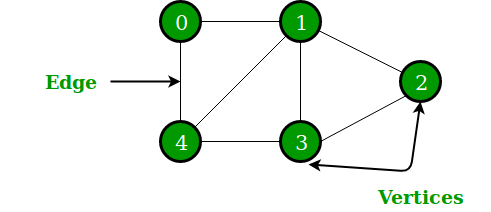
\includegraphics[width =.8 \textwidth]{graf.png}

    \caption{\emph{Figura 7: Exemple de graf. Font: \url{https://www.geeksforgeeks.org/difference-between-graph-and-tree/}}}
\end{center}

Per exemple, en el graf de la figura 7, els nodes són [0, 1, 2, 3, 4] i les arestes connecten els nodes [0-1, 0-4, 1-2, 1-3, 1-4, 2-3, 3-4]. \newline

Els grafs s'utilitzen recurrentment per resoldre problemes de la vida real i poden representar camins, carreteres, xarxes, etc.
Com a exemple de l'ús dels grafs a la vida quotidiana trobem les xarxes socials com Instagram, Facebook, etc. Cada usuari es representa com a un node que conté una estructura on es guarden les seves dades (id, nom, gènere, gustos, etc.) i a la vegada, aquest node està connectat amb altres nodes (seguidors, contactes, amics, etc.) mitjançant arestes. \newline

Un graf és connex si existeix un camí entre dos nodes qualssevol i no ho és si no es pot anar a un node qualsevol des d'un node inicial. \newline

\begin{center}
    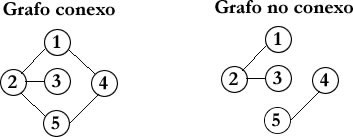
\includegraphics[width=.7 \textwidth]{GrafoConexo.jpg}

    \caption{\emph{Figura 8: Graf connex i graf no connex. Font: \url{https://www.unipamplona.edu.co/unipamplona/portalIG/home_23/recursos/general/11072012/grafo3.pdf}}}
\end{center}

\newpage

A la figura 8, apreciem que en el graf connex, podem anar a un node qualsevol des de qualsevol altre node, ja que tots els nodes estan connectats per arestes, en canvi, en el graf no connex contemplem que no podem anar a qualsevol node des de qualsevol altre node inicial. Per exemple, no es pot anar al node 5 des del node 1, puix que no hi ha un camí de nodes connexos units per arestes pels quals puguem assolir el node 5. \newline

A la figura 8, el graf connex consta d'una sola component connexa: [1,2,3,4,5].

A la figura 8, el graf no connex consta de dos components connexes: [1,2,3] i [4,5]. \newline \newline

Un graf conté un cicle si existeix algun recorregut o camí on el node inicial i el final sigui el mateix i sempre que ambdós nodes no siguin adjacents, és a dir, no estiguin connectats per una aresta. \newline

\begin{center}
    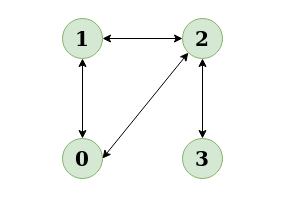
\includegraphics[width=.5 \textwidth]{GrafCicle.png}

    \caption{\emph{Figura 9: Graf amb cicle. Font: Propia}}
\end{center}

A la figura 9, observem que el graf conté un cicle, ja que podem fer el següent recorregut 0 -> 1 -> 2 -> 0 i, per tant, el node inicial i el final coincideixen (0), aquest fet causa que puguem entrar en un bucle infinit. \newline \newline

Un graf és un arbre si consta de $n$ nodes i $n-1$ arestes i no conté cap cicle, per tant, podem deduir que tan sols existeix un camí possible entre dos nodes qualsevols.

\begin{center}
    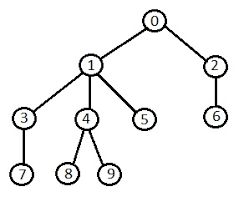
\includegraphics[width=.4 \textwidth]{TreeRoot.png}

    \caption{\emph{Figura 10: Graf (arbre). Font: \url{https://www.chegg.com/homework-help/questions-and-answers/consider-tree-tfe1png-answer-following-1-tis-rooted-vertex-2-siblings-vertex-3-3-parent-ve-q54883116}}}
\end{center}

Existeixen dues variacions de les arestes en els grafs: \newline

\textbf{Graf no dirigit:} les arestes del graf connecten dos nodes qualssevol per les dues bandes, és a dir, donats dos nodes $x$ i $y$, els quals estan connectats per una aresta, es pot anar tant des del node $x$ fins al $y$ com des del node $y$ fins al $x$, per tant, el graf es pot recórrer des de qualsevol node.

(Les arestes d'un graf no dirigit ens les podem imaginar com carreteres de doble sentit).
\newline

\textbf{Graf dirigit:} les arestes del graf només es poden recórrer en una direcció, és a dir, existeix una connexió entre els nodes x->y, però no entre y->x.

(Les arestes d'un graf no dirigit ens les podem imaginar com carreteres d'un únic sentit).

\begin{center}
    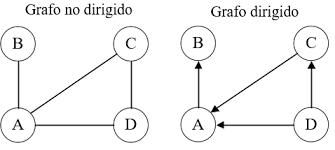
\includegraphics[width=.7 \textwidth]{GrafDir.png}
    
    \caption{\emph{Figura 11: Graf dirigit i graf no dirigit. Font: \url{https://www.researchgate.net/figure/Ejemplos-de-un-grafo-dirigido-y-un-grafo-no-dirigido_fig7_309278789}}}
\end{center}

Podem observar a la imatge que en el graf no dirigit, podem anar a qualsevol node des de qualsevol node, en canvi, en el graf dirigit, des del node B no poden anar enlloc jas que no disposa de cap connexió amb cap node. \newline

Per recórrer els grafs hi ha dos algorismes fonamentals: la cerca en profunditat, més coneguda com a DFS (depth-first search) o la cerca en amplada, més coneguda com a BFS (breadth-first search).

Els dos algorismes parteixen des d'un node inicial i després recorren tots els nodes als quals es poden arribar a partir d'aquest node inicial.

La diferència entre els dos algorismes és l'ordre amb el qual es recorren els nodes.

El que canvia entre la cerca en profunditat i la cerca en amplada i que en conseqüència provoca que l'ordre de visitar els nodes sigui diferent, és l'estructura de dades que utilitzen, la cerca en profunditat utilitza un stack (pila) o la recursió, en canvi, la cerca en amplada utilitza una queue (cua).

